\section{2016}
\subsection{}

What are the Fourier coefficients $C_{-1}$, $C_{0}$ and $C_{1}$ of the exponential Fourier series for the function below?

\begin{equation}
  f(x)=2+cos(2 \pi x)
\end{equation}




\subsection{}

Considering the periodic squarewave described by the function

\begin{equation}
    f(t)=
    \begin{cases}
        0 & \text{for } 0<t<1 \\
        -1 & \text{for } 1<t<2
    \end{cases}
\end{equation}

\begin{center}
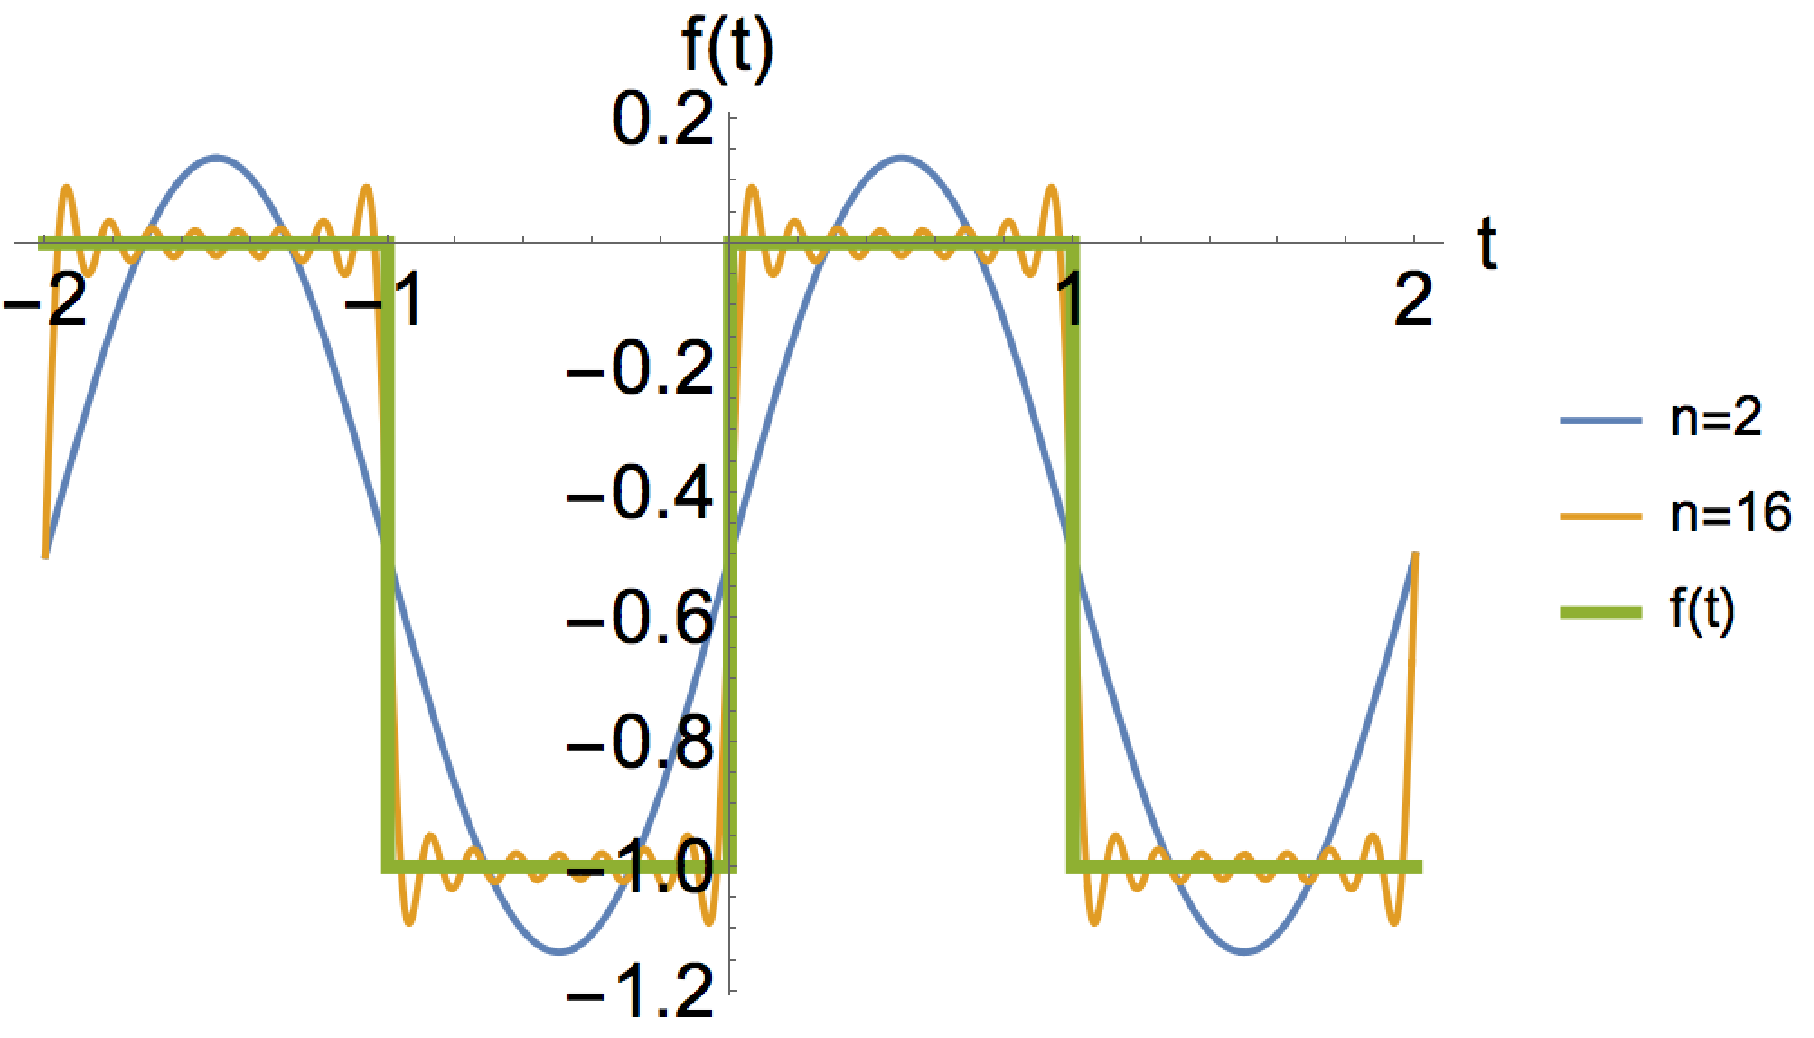
\includegraphics[scale=0.75]{fourier_series_square_wave_midtermexam.png}
\end{center}

1. Calculate the Fourier coefficient $C_0$.

2. Obtain an expression for the Fourier coefficients $C_k$ where $k \ne 0$. Write your final answer so that it does not contain any exponentials, sines or cosines.

3. What is Gibb's phenomenon? Under what situations does it occur?




\subsection{}

In the first lecture we saw that it was possible to make any function (such as the ``Homer Simpson'' function) by taking a point and rotating it around a circle that itself was rotating around a larger circle, that itself was rotating around a larger circle, and so on. This is also how the ancient greeks tried to approximate the orbit of the planets and sun around the earth.

1. How is the ability to approximate an arbitrary function using sums of circles related to Fourier series? You may refer to the equation
\begin{equation}
    f(t) = \sum_{k=-N}^{k=N} C_k e^{2 \pi i k t}
\end{equation}
during your discussion.

2. By what variables are frequencies and radii of the circles defined in the Fourier series in the above equation?

3. The terms of the Fourier series are orthogonal. Describe in a few sentences what this means. You may refer to the below expression in your answer.
\begin{equation}
    (e^{2 \pi i k_1 t},e^{2 \pi i k_2 t})
\end{equation}
